% !TeX spellcheck = it_IT
\documentclass{article}



\usepackage{arxiv}

\usepackage[utf8]{inputenc} % allow utf-8 input
\usepackage[T1]{fontenc}    % use 8-bit T1 fonts
\usepackage{hyperref}       % hyperlinks
\usepackage{url}            % simple URL typesetting
\usepackage{booktabs}       % professional-quality tables
\usepackage{amsfonts}       % blackboard math symbols
\usepackage{nicefrac}       % compact symbols for 1/2, etc.
\usepackage{microtype}      % microtypography
\usepackage{lipsum}		% Can be removed after putting your text content
\usepackage{listings}
\usepackage{url}
\usepackage{graphicx}
\usepackage{longtable}
\usepackage{float}

\renewcommand{\figurename}{Figura}
\renewcommand{\tablename}{Tabella}
 
\lstset{
   basicstyle=\ttfamily\footnotesize
}  

\title{Analisi di un'applicazione grafica in ambiente erika³}

%\date{September 9, 1985}	% Here you can change the date presented in the paper title
%\date{} 					% Or removing it

\author{
  Stefano Panozzo\\
  Dipartimento di Matematica\\
  Università di Padova, Italia I-35121\\
  \texttt{Email: stefano.panozzo.1@studenti.unipd.it} \\
  %% examples of more authors
  %% \AND
  %% Coauthor \\
  %% Affiliation \\
  %% Address \\
  %% \texttt{email} \\
  %% \And
  %% Coauthor \\
  %% Affiliation \\
  %% Address \\
  %% \texttt{email} \\
  %% \And
  %% Coauthor \\
  %% Affiliation \\
  %% Address \\
  %% \texttt{email} \\
}

% Uncomment to remove the date
\date{}

% Uncomment to override  the `A preprint' in the header
\renewcommand{\headeright}{}
\renewcommand{\undertitle}{Relazione Tecnica}

\begin{document}
\maketitle

\begin{abstract}
Questa relazione descrive un'applicazione \textit{real-time} sviluppata con il supporto di ERIKA³, un \textit{Hard Real Time Operating System (RTOS)} certificato OSEK/VDX in utilizzo in ambito automobilistico. L'applicazione consiste in diversi \textit{task} che competono fra loro per raggiungere un obiettivo \textit{target}. L'applicazione è testata in diverse configurazioni e condizioni di carico per vedere come queste influenzino l'esecuzione del sistema; in particolare utilizzo come metrica il numero di errori di attivazione dei \textit{task}, equiparabili a \textit{deadline-miss} quando un \textit{task} supporta una sola attivazione e le \textit{deadline} sono implicite.
\end{abstract}


% keywords can be removed
% \keywords{First keyword \and Second keyword \and More}
\section{Introduzione}
I sistemi \textit{embedded} sono di utilizzo comune nella vita di tutti i giorni: dai semplici sensori domotici nelle case ai più complessi sistemi che controllano un'automobile. Se però nei primi può non vedersi la necessità di garantire che il sistema funzioni sempre nel modo corretto e leggeri ritardi nell'esecuzione dei compiti sono ammissibili, in un sistema complesso che svolge compiti critici che coinvolgono direttamente la persona risulta necessaria la comprensione di ciò che accade oltre a ciò che ci è immediatamente visibile.

Al giorno d'oggi le automobili si possono considerare l'oggetto nella vita di tutti i giorni più tecnologicamente avanzato. Basti pensare all'enormità di sensori che sono presenti nei veicoli di ultima generazione: dai dispositivi per la sicurezza del passeggero, come l'ABS o il \textit{lane assist}, ai sistema di intrattenimento di bordo. E se pensiamo al futuro, l'utilizzo di tecnologie sempre più avanzate non diminuirà, come ad esempio i sistemi a guida autonoma o la comunicazione tra veicoli o tra un veicolo e l'infrastruttura presente lungo la strada. Si riesce quindi a capire come sia necessario gestire tutti questi sistemi in modo tale da mantenere un certo ordine e garantire che sistemi a criticità massima, come quelli relativi alla sicurezza del passeggero, non siano disturbati da un malfunzionamento di sistemi secondari non critici, e che quindi sia necessario garantire che alcuni vincoli durante tutta l'esecuzione del sistema siano soddisfatti.

Per questo motivo, nel corso degli anni, sono nati degli standard per garantire un modello omogeneo di architettura software in ambito \textit{automotive}, partendo dal più vecchio standard OSEK/VDX\footnote{\url{https://web.archive.org/web/20160307021413/http://osek-vdx.org/}} alle nuove versioni di AUTOSAR\footnote{\url{https://www.autosar.org/}}.

Erika³\footnote{\url{http://erika-enterprise.com/}} è un \textit{Hard Real Time Operating System (RTOS)} che implementa le funzionalità richieste dagli standard sopracitati, fornendo delle primitive che semplificano lo sviluppo e offrono un livello di astrazione rispetto all'hardware sottostante.

Per lo svolgimento di questa analisi ho quindi scelto l'utilizzo di Erika³ su una \textit{bare-board} STM32F429I-Discovery\footnote{\url{https://www.st.com/en/evaluation-tools/32f429idiscovery.html}}, un kit per lo sviluppo \textit{low-cost} con un microcontrollore STM32F4 e un \textit{core} ARM Cortex-M4.

\section{ERIKA³}
Come già detto, Erika³ supporta lo standard OSEK/VDX, il che comporta delle scelte progettuali ben definite.

\subsection{Fixed-priority scheduling}
In questo tipo di \textit{scheduling}, ogni \textit{task} ha una priorità fissata e statica, determinata \textit{offline}. La priorità di un \textit{task} deriva dai suoi parametri temporali, quindi non ha direttamente a che fare con la sua importanza relativa per l'integrità del sistema (criticità).

Un \textit{task} rappresenta l'unità architetturale di lavoro da svolgere, ossia il compito che il sistema deve fare, che viene poi realizzato dal \textit{job}, ovvero ciò che il sistema (o meglio lo \textit{scheduler}) fa eseguire a \textit{runtime}. Un \textit{job}, di conseguenza, eredita la priorità del task che lo definisce.

Durante l'esecuzione il \textit{job} a priorità più alta viene eseguito, mentre gli altri attendono finchè non ci sarà più nessun \textit{job} a priorità maggiore nella coda dei pronti.

Per assegnare la priorità dei \textit{task} si possono seguire due strategie:

\begin{itemize}
	\item \textit{Rate monotonic}: il \textit{task} con periodo minore (il cui \textit{job} viene attivato più frequentemente) ha priorità maggiore; il rate di un \textit{task} è l'inverso del periodo.
	\item \textit{Deadline monotonic}: il \textit{task} con la \textit{deadline} relativa più vicina ha priorità maggiore.
\end{itemize}

Quando la \textit{deadline} di un \textit{task} è implicita (i.e. \textit{deadline} = periodo), le due strategie si equivalgono. Quando però la \textit{deadline} non è implicita, l'algoritmo \textit{deadline monotonic} offre prestazioni migliori, nel senso che può produrre, entro certi limiti, uno \textit{schedule feasible} anche quando non è possibile con \textit{rate monotonic}.

\textit{Fixed-priority scheduling} supporta il prerilascio, ovvero se mentre un \textit{job} esegue viene aggiunto alla coda dei pronti un altro \textit{job} a priorità maggiore, il primo può essere interrotto e, dopo aver effettuato il \textit{context switch}, il secondo viene fatto eseguire.

\subsection{Shared/Private stack e Immediate Priority Ceiling}
Una delle particolarità dei sistemi \textit{embedded} è la carenza di memoria RAM. È fondamentale quindi attuare soluzioni che preservino il più possibile questo tipo di memoria.

Per fare ciò si può optare per uno \textit{stack} condiviso fra due o più \textit{task}, in modo da ottimizzare la memoria allocata staticamente a questi. Così facendo, la memoria utilizzata dai \textit{task} non in esecuzione sarà libera ed utilizzabile dagli altri.

Guardando la Figura \ref{interlived-execution} e ragionando sul funzionamento dello \textit{stack}, si capisce però che uno \textit{stack} condiviso, quando lo \textit{scheduling} permette il prerilascio, può portare problemi. 

\begin{figure}[!htbp]
	\centering
	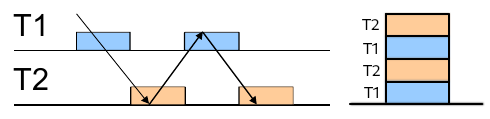
\includegraphics[width=2in]{image/Interleaved_execution-stack.png}
	\caption{\textit{Interleaved Execution} e stato dello \textit{stack} dopo il secondo prerilascio di T1}
	\label{interlived-execution}
\end{figure}

Essendo l'ordinamento dello \textit{stack} di tipo FIFO, nel caso di \textit{stack} condiviso e \textit{interleaved execution}, si avrebbe una frammentazione dello \textit{stack}.

Per capire quando può avvenire una situazione del genere, bisogna ragionare su quando un \textit{task} può essere sospeso per farne eseguire un altro. Oltre all'arrivo di un \textit{task} a priorità maggiore, un \textit{task} può essere sospeso se, ad esempio, non può accedere ad una risorsa necessaria per procedere perchè in possesso di un altro \textit{task}. Questo problema può portare anche a \textit{priority inversion}, dove un \textit{task} a priorità più alta è bloccato da un \textit{task} a priorità più bassa perchè in possesso di una risorsa necessaria per procedere. Questo problema è illustrato nella Figura \ref{priority-inversion}, in cui T1 ha una \textit{deadline miss}, e in cui l'ordine delle priorità è T1>T2>T3.

\begin{figure}[H]
	\centering
	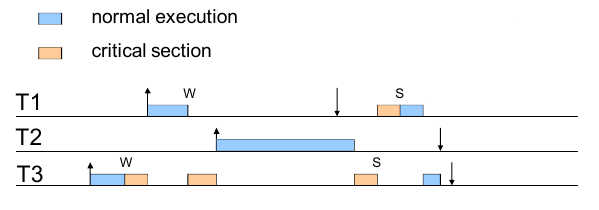
\includegraphics[width=4in]{image/Priority_inversion.png}
	\caption{\textit{\textit{Priority Inversion}}}
	\label{priority-inversion}
\end{figure}

Per evitare questo problema e mantenere il prerilascio, si può adottare un algoritmo che permetta, una volta ottenuto l'utilizzo della risorsa, di eseguire senza essere interrotti da un altro \textit{job} che necessita della stessa. Nello standard OSEK/VDX si è scelto di optare per \textit{Immediate Priority Ceiling Protocol}, che permette di inibire il prerilascio nelle sezioni critiche di \textit{job} in cui si utilizza una risorsa condivisa. Questo grazie al fatto che, quando un \textit{job} ottiene una risorsa libera, aumenta la sua priorità al \textit{priority ceiling} di questa, definita come la priorità del \textit{task} a priorità maggiore che la utilizza. Così facendo, il \textit{job} in esecuzione non potrà mai essere interrotto da un altro \textit{job} durante la sezione critica.

\subsection{OIL File}
Lo standard OSEK/VDX impone un approccio statico, ovvero ogni specifica deve essere nota \textit{offline}, prima che il sistema cominci l'esecuzione. Il file OIL è dove queste specifiche, rappresentanti la configurazione del \textit{kernel}, sono definite.

Gli oggetti le cui proprietà sono definite nel file OIL sono i seguenti:
\begin{itemize}
	\item CPU: la CPU su cui l'applicazione esegue;
	\item OS: specifiche del sistema operativo che esegue;
	\item ISR: \textit{Interrupt Service Routine} supportate dal sistema operativo;
	\item RESOURCE: le risorse che possono essere usate da un \textit{task};
	\item TASK: la configurazione dei \textit{task} gestiti dal sistema operativo;
	\item COUNTER: rappresenta il \textit{tick} che attiva gli allarmi. Può essere hardware o software;
	\item EVENT: gli eventi definiti per un \textit{task};
	\item  ALARM: gli allarmi che vengono attivati da un \textit{counter}; quando azionati, possono attivare \textit{task}, invocare funzioni di \textit{callback} o cambiare lo stato di un evento;
	\item MESSAGE: il messaggio COM che fornisce la comunicazione locale o di rete;
	\item COM: il sottosistema di comunicazione inter- and intra- ECU;
	\item NM: il sottosistema per il \textit{network management}.
\end{itemize}
Esiste inoltre una suddivisione in categorie di alcuni servizi che il sistema offre:
\begin{itemize}
	\item TASK - I \textit{task} possono essere di quattro categorie differenti, definite \textit{Conformance Classes}:
	\begin{enumerate}
		\item BCC1: il tipo più semplice di \textit{task} (\textit{Basic task}), consente una sola attivazione (i.e. se un \textit{job} viene attivato mentre il \textit{task} non è nello stato \textit{suspended}, questa nuova attivazione viene persa) e un \textit{task} per priorità;
		\item BCC2: \textit{Basic task} ma con la possibilità di attivazioni multiple (le nuove attivazioni rimangono pendenti finchè il vecchio \textit{job} non termina) e più di un \textit{task} per priorità;
		\item ECC1: analogo al BCC1, ma la classe di \textit{Extended task} consente la gestione degli eventi;
		\item ECC2: \textit{Extended task} ma con la possibilità di attendere eventi multipli e più di un \textit{task} per priorità.
	\end{enumerate}
	La Tabella \ref{task-class} riporta le principali differenze fra le diverse \textit{Conformance Classes}.
	\begin{table}[!htbp]
		\centering
		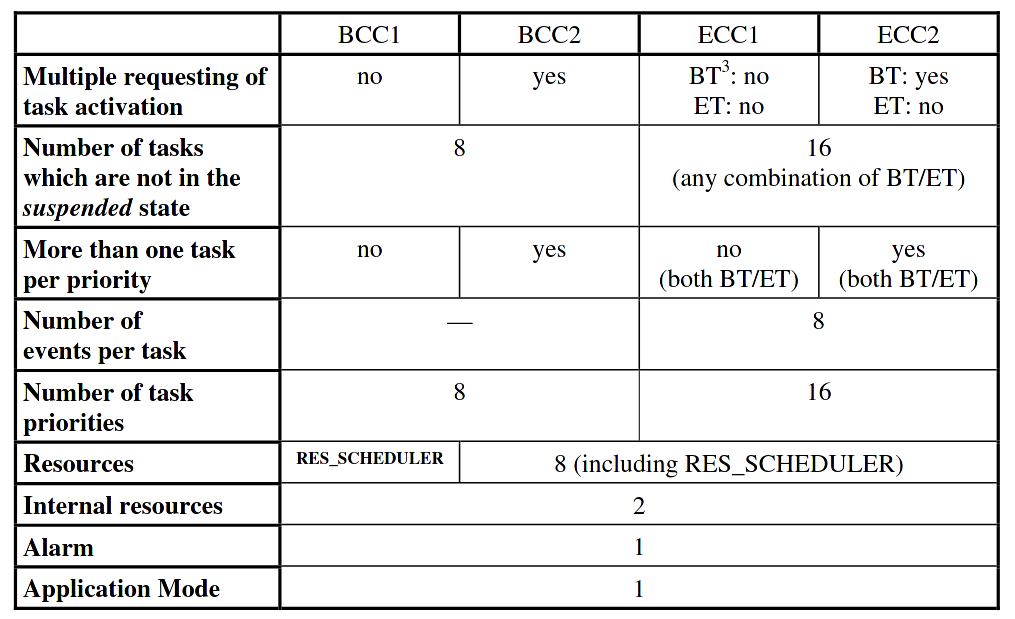
\includegraphics[width=4in]{image/Task_ConformanceClass.png}
		\caption{\textit{\textit{Conformance Classes - Fonte: OSEK 2.2.3 specification}}}
		\label{task-class}
	\end{table}
	
	Come si può intuire, aggiungendo funzionalità ad un tipo di \textit{task}, la complessità a livello di gestione da parte del sistema operativo aumenta. Ad esempio, per supportare attivazioni di \textit{task} con la stessa priorità, deve essere definita una struttura dati che mantenga l'ordine di attivazione, che poi verrà gestita dallo \textit{scheduler} secondo l'ordinamento FIFO.
	
	La maggiore complessità si può intuire anche valutando i possibili stati in cui \textit{Basic \textit{task}} ed \textit{Extended \textit{task}} possono essere, come riportato nella Figura \ref{states}.
	\begin{figure}[!htbp]
		\centering
		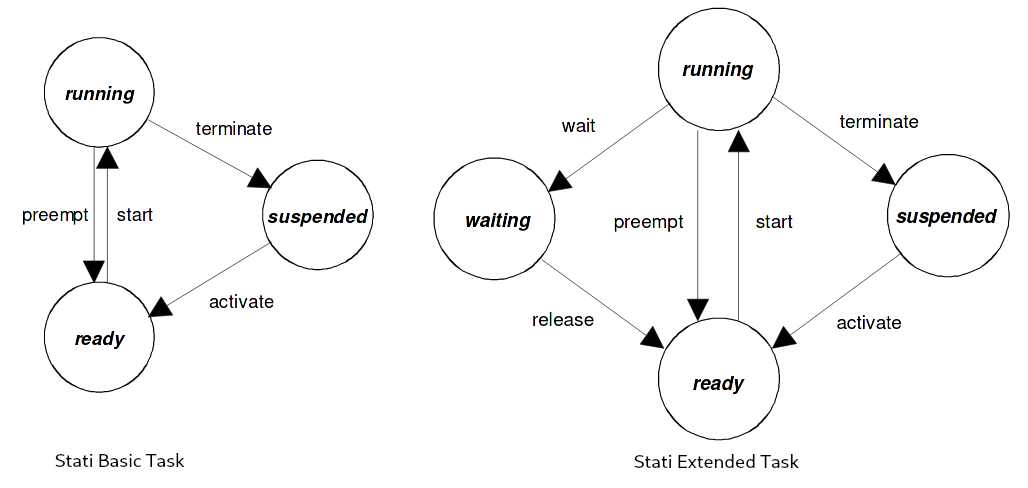
\includegraphics[width=4in]{image/States.png}
		\caption{\textit{Possibili stati nelle diverse classi - Fonte: OSEK 2.2.3 specification}}
		\label{states}
	\end{figure}
	\item Interrupt - sono suddivisi in due categorie differenti:
	\begin{enumerate}
		\item ISR1: interrupt che non effettuano chiamate a primitive di sistema e, una volta terminati, l'esecuzione prosegue esattamente da dove era stata interrotta;
		\item ISR2: interrupt più complessi dei precedenti, possono effettuare chiamate a delle primitive di sistema e, proprio per questa capacità, al termine dell'esecuzione viene invocato lo \textit{scheduler}.
	\end{enumerate}
	Gli ISR1 hanno priorità sempre maggiore degli ISR2, infatti i primi possono interrompere anche operazioni del \textit{kernel}, mentre i secondi vengono eseguiti in seguito alla terminazione di queste.
\end{itemize}
Qualsiasi sia la priorità dei servizi offerti dall'OS, il compilatore assicura che ci sia un ordine ben preciso a \textit{runtime} durante l'esecuzione di questi. Risulta quindi che gli interrupt avranno sempre la precedenza sui \textit{task}, e gli ISR1 avranno a loro volta la precedenza sugli ISR2, come si può vedere dalla Figura \ref{processing-levels} .
\begin{figure}[H]
	\centering
	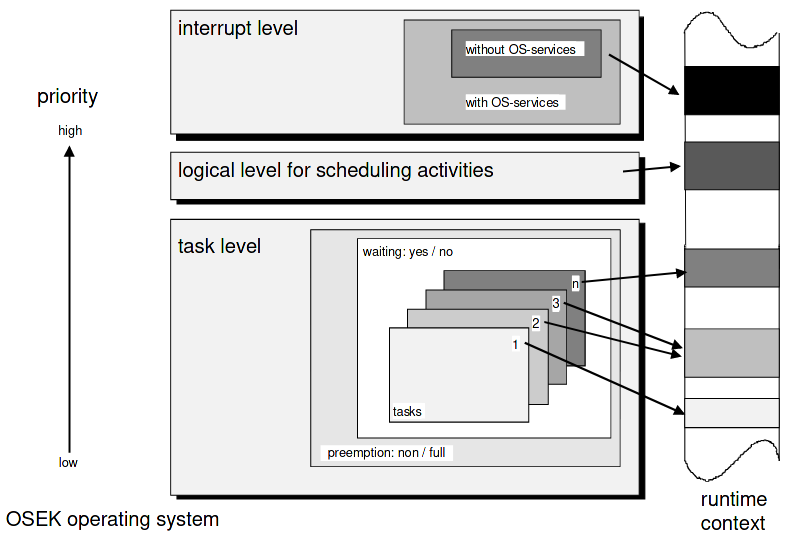
\includegraphics[width=4in]{image/Priority_levels.png}
	\caption{\textit{\textit{Processing Levels} - Fonte: OSEK 2.2.3 specification}}
	\label{processing-levels}
\end{figure}

\section{Applicazione}
L'applicazione proposta utilizza quindi ERIKA³ e lo standard OSEK/VDX. Oltre a ciò, utilizza anche il \textit{framework} TouchGFX\footnote{\url{https://support.touchgfx.com/docs/introduction/welcome}}, che aiuta lo sviluppo di interfacce grafiche complesse per sistemi hardware basati su microcontrollori STM32. Questo \textit{framework} mantiene sincronizzata l'interfaccia grafica del display con il modello dei dati rappresentanti gli oggetti sullo schermo e comunica eventuali interazioni con essi attraverso il \textit{touchscreen}.

L'applicazione di test consiste in un \textit{task} che genera un punto target sullo schermo, indicato tramite un cerchio rosso, e tre \textit{task} (o sei in base al test) con parametri di configurazione e implementazione differenti che lo devono raggiungere.
È di interesse capire come l'applicazione e il sistema reagiscono all'aumentare delle interferenze e in differenti condizioni di carico. Mi attendo quindi un rallentamento della reattività del sistema e nello specifico, in base alle differenti configurazioni, una visibile differenza nello spostamento dei giocatori visualizzati a schermo che rappresentano i \textit{task} del sistema.

Per avere una valutazione quantitativa e analizzare quello che accade a schermo, come metrica di confronto fra le varie configurazioni utilizzo il numero di \textit{deadline miss} dei \textit{task}, misurata con l'ausilio della primitiva \textit{ErrorHook} in seguito definita. Tramite questa, infatti, è possibile sapere e gestire quando un nuovo \textit{job} viene attivato, ad esempio da un allarme, mentre un vecchio \textit{job} dello stesso \textit{task} è ancora attivo (i.e. non nello stato \textit{suspended}). Con la condizione di \textit{deadline} implicite e \textit{task} attivati solamente da allarmi periodici, questo significa che il vecchio \textit{job} ha una \textit{deadline miss}. In seguito chiamo questi eventi errori di attivazione. 
Tramite questa metrica, quindi, cercherò di valutare il comportamento del sistema nell'insieme e in seguito, più nello specifico, quali sono i \textit{task} che subiscono più interferenze.

\subsection{Configurazione del sistema}
La \textit{conformance class} dei \textit{task} del sistema è di tipo ECC1, in quanto il \textit{task} che gestisce l'interfaccia grafica non termina mai e rimane in attesa di eventi che notificano un nuovo \textit{framebuffer} per aggiornare il display.
Di seguito riporto la definizione del Task1, che si occupa della gestione dell'interfaccia grafica.
\begin{lstlisting}[language=C]
1  TASK Task1 {
2	 PRIORITY = 3;               /* Priorita del task */
3	 ACTIVATION = 1;             /* Numero di attivazioni supportate */
4	 SCHEDULE = FULL;            /* Task prerilasciabile */
5	 AUTOSTART = TRUE;           /* Attivazione allo startup del sistema */
6	 STACK = PRIVATE {           /* Stack privato e relativa dimensione */
7	 	SIZE = 4096;
8	 };
9	 EVENT = FrameBufferEvent;   /* Supporto all'evento 'FrameBufferEvent' */
10	 EVENT = VSyncEvent;         /* Supporto all'evento 'VSyncEvent' */
11	 RESOURCE = HalResource;     /* Utilizzo della risorsa 'HalResource' */
12 };
\end{lstlisting}
Gli eventi dichiarati per questo \textit{task} sono necessari per mantenere sincronizzato il display e l'\textit{engine}, e per supportare questi è necessario quindi che il suo \textit{stack} sia privato. Il numero di attivazioni supportate si riferisce a cosa accade quando viene attivato il \textit{task} se questo è già in esecuzione: la configurazione scelta (una sola attivazione) implica che ogni attivazione pone il \textit{task} nello stato \textit{ready} solamente se quel \textit{task} non è già attivo, altrimenti l'attivazione è persa.

Gli altri \textit{task} presenti nel sistema sono:
\begin{itemize}
	\item TaskBackground: ha priorità minima e non termina mai, per queste caratteristiche esegue solamente quando nessun altro \textit{task} deve eseguire. È utile per il calcolo di utilizzo della CPU;
	\item Task2, Task3, Task4: rappresentano i \textit{player} dello studio;
	\item Task5, Task6, Task7: rappresentano gli eventuali \textit{player} aggiuntivi (non presenti in ogni condizione di test);
	\item Task0: rappresenta il target che i \textit{player} devono raggiungere.
\end{itemize}
Tutti questi \textit{task} hanno una configurazione di base simile: \textit{stack} condiviso e un'unica attivazione (come per il Task1), ma cambiano nelle varie prove di questo studio in base al supporto o meno al prerilascio ed eventuali \textit{offset} dall'inizializzazione del sistema.

Oltre alla configurazione dei \textit{task}, serve definire i COUNTER necessari, in questo caso solamente uno che mantenga il \textit{timing} del sistema:
\begin{lstlisting}[language=C]
1  COUNTER SystemTimer {
2	  MINCYCLE = 1;                
3	  MAXALLOWEDVALUE = 65535;    
4	  TICKSPERBASE = 1;            
5	  TYPE = HARDWARE {          
6		  SYSTEM_TIMER = TRUE;
7		  PRIORITY     = 9;         
8		  DEVICE       = "SYSTICK";
9	  };
10	  SECONDSPERTICK = 0.001; 
11  };
\end{lstlisting}
Come si può notare, ogni tick di sistema corrisponderà ad un tick hardware ogni millisecondo.
Sono definiti anche gli allarmi che definiscono le \textit{release} dei vari \textit{task}:
\begin{lstlisting}[language=C]
1  ALARM AlarmTask2 {
2	  COUNTER = SystemTimer;
3	  ACTION = ACTIVATETASK { TASK = Task2; };
4	  AUTOSTART = TRUE { ALARMTIME = 20; CYCLETIME = 10; };
5  };
\end{lstlisting}
Un esempio è l'ALARM per il Task2, attivato dal SystemTimer, in questo esempio a partire da 20ms rispetto all'inizializzazione del sistema e, in seguito, riattivato ogni 10ms.

Oltre a questi sono definiti anche tutti gli ISR1 e ISR2 necessari per la sincronizzazione e comunicazione del microcontrollore con il display, dell'invio dei dati dalla \textit{board} all'esterno tramite seriale e dell'utilizzo del pulsante fisico presente sulla \textit{board}.

Per trasmettere i dati di \textit{log} dalla \textit{board} all'esterno nel modo più efficiente possibile, ho deciso di implementare una coda circolare che trasmette tramite il modulo DMA (\textit{Direct Memory Access}). Così facendo, l'utilizzo della CPU è limitato al massimo, in quanto è necessario il suo intervento solamente al termine della trasmissione del flusso dati, all'attivazione del relarivo \textit{interrupt}. In questo modo riesco a sfruttare al meglio l'intera banda disponibile sulla \textit{board} per la trasmissione UART senza interferire significativamente sull'esecuzione del sistema.

L'inserimento dei dati nella coda circolare è effettuata direttamente dai \textit{task} o tramite i vari \textit{hook} di sistema, definiti nello standard OSEK/VDX e implementati da ERIKA³. Quelli utilizzati in questo progetto sono:
\begin{itemize}
	\item StartupHook: viene attivato al termine dell'inizializzazione dell'OS, prima che esegua lo \textit{scheduler};
	\begin{figure}[H]
		\centering
		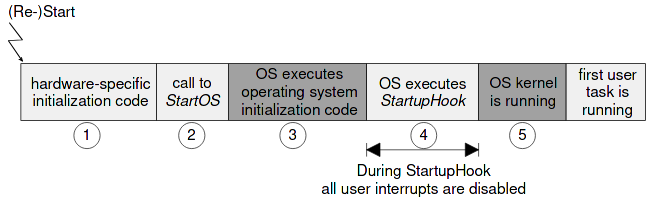
\includegraphics[width=4in]{image/StartupHook.png}
		\caption{\textit{\textit{StartupHook} - Fonte: OSEK 2.2.3 specification}}
		\label{startup}
	\end{figure}
	\item PreTaskHook e PostTaskHook: vengono eseguiti rispettivamente prima e dopo l'esecuzione di un \textit{task}. Entrambi vengono eseguiti subito dopo o prima che un \textit{task} entri o esca dallo stato \textit{running}, quindi, quando invocati, è possibile ottenere il \textit{task} a cui si riferiscono. Da precisare che questi, facendo riferimento allo stato \textit{running} di un \textit{task}, vengono invocati anche quando un \textit{task} viene prerilasciato o ritorna ad eseguire, e non solo quando è attivato inizialmente o termina. Questo risulta molto utile per il \textit{log} dei \textit{task} TaskBackground e Task1 (GUI);
	\begin{figure}[H]
		\centering
		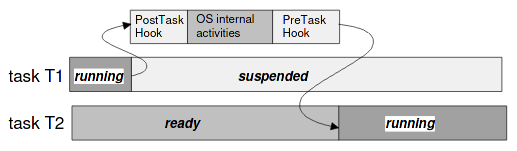
\includegraphics[width=4in]{image/PrePostTaskHook.png}
		\caption{\textit{\textit{PreTaskHook} e \textit{PostTaskHook} - Fonte: OSEK 2.2.3 specification}}
		\label{taskHook}
	\end{figure}
	\item ErrorHook: viene eseguito ogni qualvolta ci siano errori del sistema operativo, sia temporanei che fatali.  È possibile gestire differenti tipi di errore, in base allo '\textit{StatusType error}' che l'ha generato. Nello studio in questione, definito che ogni \textit{task} supporta una sola attivazione e ogni \textit{task} ha \textit{deadline} implicita uguale al periodo, è di interesse sapere quando l'ErrorHook riporta un errore di tipo 'E\_OS\_LIMIT', che viene invocato ogni qual volta viene eseguita un'attivazione di un \textit{task} già in esecuzione. In questo modo si può determinare se un \textit{task} non ha terminato entro la \textit{deadline}.
\end{itemize}
Ho quindi utilizzato PreTaskHook, PostTaskHook ed ErrorHook per il \textit{log} del sistema per avere un \textit{\textit{timestamp}} dell'esecuzione di alcuni \textit{task} e per identificare eventuali \textit{deadline-miss}.

\subsection{Test}
Ho testato il sistema in differenti condizioni, suddivisibili in base al loro scopo in due categorie:
\begin{enumerate}
	\item Test del sistema senza carico, ovvero mantenendo la computazione dei \textit{task} ridotta ma analizzando come, diminuendo il \textit{release time} fra un \textit{job} e il successivo, il sistema reagisce;
	\item Test del sistema all'aumentare delle interferenze, che possono essere causate da altri \textit{task} o dalla pressione del pulsante esterno e quindi dall'azionamento del relativo ISR2 che attiva il Task0. Si mantiene dunque costante il \textit{timing} di attivazione dei \textit{task} ma si valuta come al variare del carico dei \textit{task} o delle pressioni esterne il sistema viene perturbato.
\end{enumerate}
Per ogni test ho memorizzato, trasmettendo tramite DMA, i dati in un file di log esterno, comprendente un id incrementale della entry, il \textit{task} che ha eseguito o l'eventuale errore relativo ad un \textit{task}, il \textit{timestamp} del tempo di esecuzione del \textit{task} o il \textit{timestamp} dell'errore e l'eventuale carico \% della CPU.

D'ora in poi, chiamerò \textit{player} i \textit{task} che concorrono per raggiungere le coordinate target dello schermo.
\subsubsection{Test del sistema senza carico}
Durante questo scenario ho testato il sistema per 10 secondi e ho mantenuto il carico dei \textit{player} molto esiguo. Questi infatti, avendo a disposizione le coordinate X e Y del target, devono calcolare rispetto alla loro posizione il movimento da eseguire (il \textit{player} si può muovere di un solo pixel per direzione alla volta), quindi inviare la nuova posizione al modello dei dati poi elaborato dal \textit{framework} TouchGFX.

Ho effettuato i test sia con 3 \textit{player} - e quindi 6 \textit{task} totali - sia con 6 \textit{player} - e quindi 9 \textit{task} totali. 

Come prima cosa ho testato come reagisce il sistema senza nessun \textit{offset} sui \textit{player}, ovvero quando il \textit{release time} iniziale è per tutti uguale a 0. Come si può notare dalla tabella e dalla Figura \ref{noC-noO}, la differenza nel numero di errori di attivazione fra il sistema con 3 \textit{player} e quello con 6, comincia ad essere rilevante quando il periodo dei \textit{player} risulta uguale a 2ms. Questo era prevedibile, in quanto essendo il carico sul singolo \textit{task} esiguo, con \textit{release event} ben distanziati fra loro, tutti i \textit{player} hanno il tempo necessario per eseguire. Quando invece il periodo, e di conseguenza la \textit{laxity}, ovvero quanto un \textit{job} può ancora rimanere in attesa prima di dover eseguire per completare entro la \textit{deadline}, viene ridotto al minimo, il maggior numero di \textit{player} può causare maggior interferenza che conclude in un maggior numero di errori di attivazione e di conseguenza di \textit{deadline miss}. È possibile notare come il maggior numero di \textit{player} influisca di più anche sul carico della CPU man mano che la frequenza di attivazione aumenta.
\begin{figure}[H]
	\centering
	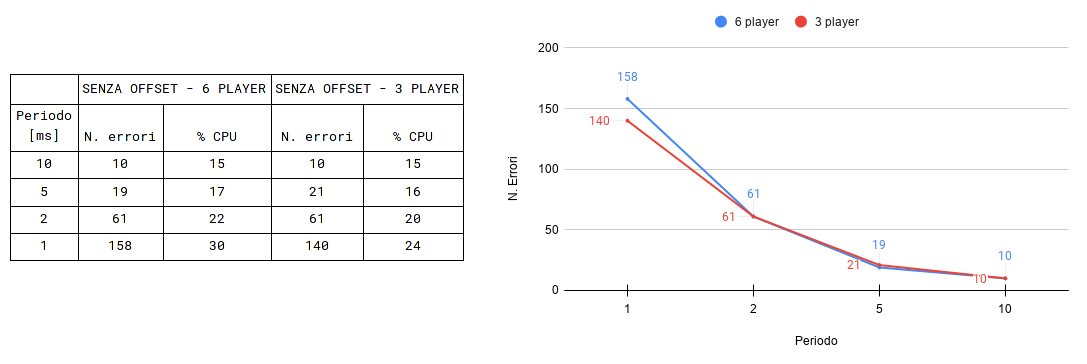
\includegraphics[width=6in]{image/NO_CARICO-AUTOSTART.png}
	\caption{Confronto \textit{deadline miss} dei \textit{task} e \% CPU con 3 e 6 \textit{player} senza \textit{offset}}
	\label{noC-noO}
\end{figure}
È inoltre testato se l'aggiunta di un \textit{offset} arbitrario possa diminuire il numero di errori e quindi di \textit{deadline miss}; in questo caso i primi release event dei \textit{player} sono stati posti a 20ms (per i \textit{player} 1 e 4), 23ms (per i \textit{player} 2 e 5) e 27ms (per i \textit{player} 3 e 6). Essendo i \textit{task} periodici, l'\textit{offset} si è poi mantenuto nel tempo anche nelle successive attivazioni.

Come si può vedere nella Figura \ref{noC-siO}, un \textit{offset} sull'attivazione dei \textit{task}, in modo che i \textit{release event} avvengano in momenti sufficientemente distanziati, migliora il numero di errori di attivazione. Con periodo uguale a 1ms mi sarei aspettato un minor miglioramento delle prestazioni, considerando che l'utilità dell'\textit{offset} è nulla se i \textit{release event} dei \textit{player} si sovrappongono perchè il periodo è minore o uguale alla differenza fra l'\textit{offset} di due \textit{task}.
\begin{figure}[H]
	\centering
	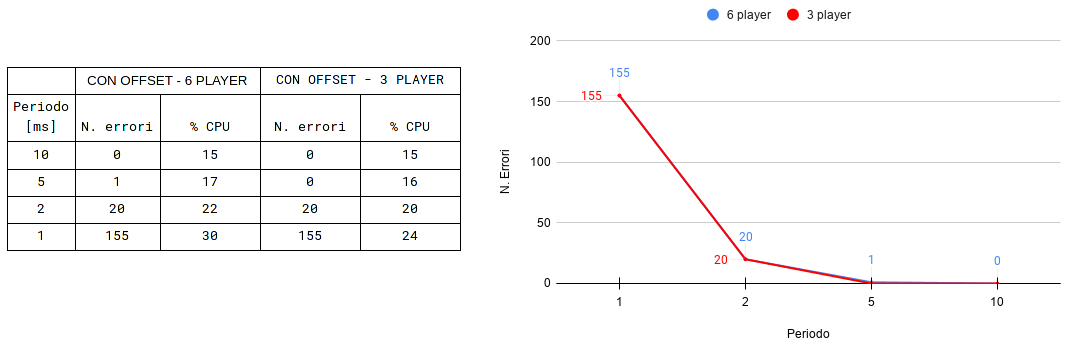
\includegraphics[width=6in]{image/NO_CARICO-OFFSET.png}
	\caption{Confronto \textit{deadline miss} dei \textit{task} e \% CPU con 3 e 6 \textit{player} con \textit{offset} arbitrario}
	\label{noC-siO}
\end{figure}

\subsubsection{Test del sistema all'aumentare del carico}
Durante questo test ho mantenuto costante a 10 ms il periodo di attivazione dei \textit{task} e ho definito solamente 3 \textit{player}, utilizzando gli \textit{offset} scelti nel precedente test. Questo perchè così facendo parto da una base in cui, senza carico, non ho ottenuto nessun errore di attivazione.

Ho invece aumentato il carico, in particolare sul \textit{player} 3, e testato se eventuali pressioni del pulsante fisico presente sulla \textit{board}, che attivano il Task0 (target), influiscono sul numero di errori di attivazione.

L'aumento del carico sul \textit{player} 3 è determinato dal semplice codice qui di seguito:
\begin{lstlisting}[language=C]
1  for(int i = 0; i < load; ++i)
2	  for(int z = 0; z < load; ++z)
3		  sum += i+z;
\end{lstlisting}
in cui la variabile 'load' rappresenta il carico sul \textit{player} 3 che viene aumentato nei vari test.
L'iterazione non viene ottimizzata dal compilatore, essendo la variabile 'sum' definita come \textit{'volatile'}.

Ho testato il sistema con prerilascio attivato per tutti i \textit{task}, con prerilascio disattivato per i \textit{player} e infine con prerilascio ma con il \textit{player} 3 con una priorità maggiore di quella degli altri \textit{player}. Negli altri due test, invece, ho assegnato  al \textit{player} 3 una priorità minore rispetto agli altri.

È importante notare come il \textit{player} 3, già con carico uguale a 300, impiega 8/9 ms per completare l'esecuzione, quindi ogni carico aggiuntivo rende il \textit{task} non \textit{feasible}. È di interesse quindi valutare come la presenza di un \textit{task} non \textit{feasible} influisce sull'intero sistema in esecuzione e se qualche configurazione aiuti a mitigare le \textit{deadline miss} totali.
\begin{figure}[H]
	\centering
	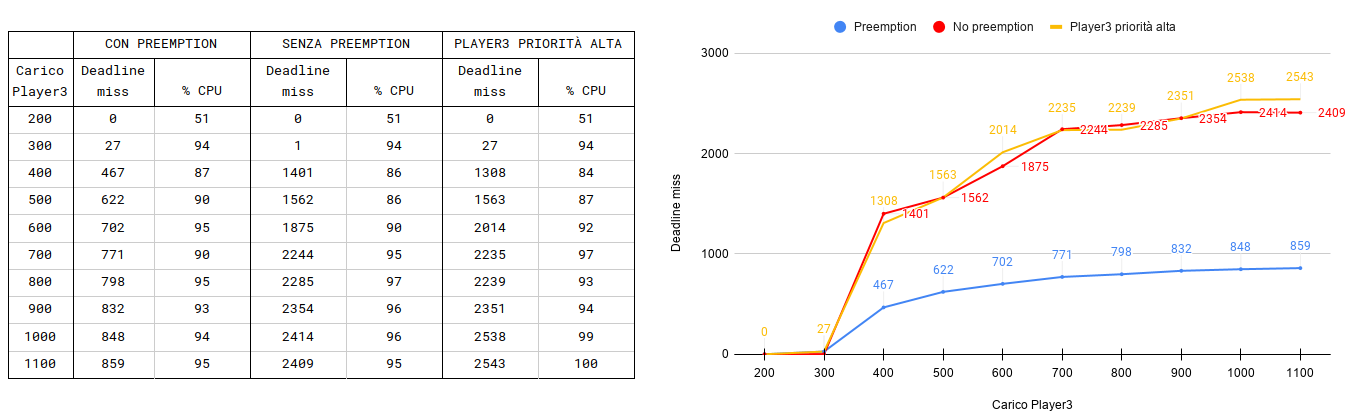
\includegraphics[width=7in]{image/CARICO-OFFSET.png}
	\caption{Confronto \textit{deadline miss} dei \textit{task} e \% CPU con \textit{preemption}, senza \textit{preemption} e con \textit{player} 3 con priorità alta, con \textit{offset} arbitrario}
	\label{siC-siO}
\end{figure}
Come si può notare dai risultati ottenuti in Figura\ref{siC-siO}, la presenza di prerilascio diminuisce di molto il numero di errori di attivazione. La differenza fra l'esecuzione senza prerilascio e con prerilascio ma con il \textit{player} 3 a priorità maggiore degli altri due \textit{player} è esigua. Questo era prevedibile, essendo il \textit{player} 3 il \textit{task} bloccante e avendo un tempo d'esecuzione molto maggiore degli altri \textit{task}. 

Si nota come il carico \% sulla CPU non mantiene un andamento lineare al crescere del carico sul \textit{player} 3 quando lo \textit{schedule} non è \textit{feasible} (carico > 300). Ciò può essere dovuto al fatto che la nuova attivazione di un \textit{task} mentre un suo vecchio \textit{job} è ancora in esecuzione causa la perdita di quella attivazione, e dunque quel task una volta terminato rimarrà in attesa di un nuovo allarme senza eseguire. È da notare, comunque, che in alcuni test con un'altra applicazione, il carico ha raggiunto un valore di picco > 100\%; ciò potrebbe indicare un errore nella libreria STM utilizzata per ottenere il valore, ma ciò non è stato approfondito.

Per completezza, ho testato il sistema anche senza utilizzare alcun \textit{offset}.
\begin{figure}[H]
	\centering
	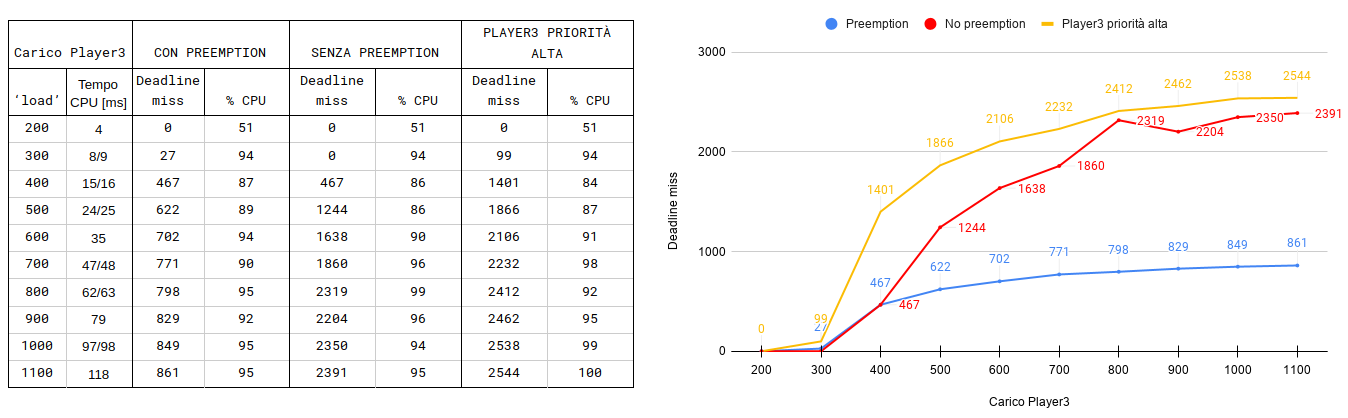
\includegraphics[width=7in]{image/CARICO-AUTOSTART.png}
	\caption{Confronto \textit{deadline miss} dei \textit{task} e \% CPU con \textit{preemption}, senza \textit{preemption} e con \textit{player} 3 con priorità alta, senza \textit{offset}}
	\label{siC-noO}
\end{figure}
La differenza più grande si nota durante l'esecuzione del sistema, visualizzando il comportamento dei \textit{player} sullo schermo. 

Con \textit{preemption} attiva, il risultato a schermo è il medesimo sia con \textit{offset} che senza: i \textit{player} 1 e 2 si muovono alla stessa velocità mentre il \textit{player} 3 risulta più lento.

Con \textit{preemption} disattivata, l'utilizzo dell'\textit{offset} mitiga l'effetto delle interferenze del \textit{player}3 sugli altri \textit{task}, in particolare sul \textit{player}2, che, con alcuni carichi, risulta visibilmente più veloce.

Con il \textit{player} 3 a priorità più alta, utilizzando l'\textit{offset} si nota lo stesso effetto precedente, mentre senza \textit{offset} il \textit{player} 3 risulta visibilmente più veloce, a conferma di un maggior numero di errori di attivazione per gli altri due \textit{player}.

La pressione del pulsante fisico non risulta causare errori di attivazione aggiuntivi, nemmeno quando l'input è stato attivato assiduamente.

Per trovare una corrispondenza fra ciò che si nota a schermo e quello che accade nel sistema sottostante, ho cercato di analizzare quali \textit{task} subiscono maggiori interferenze, suddividendo le \textit{deadline miss} per ogni \textit{task}. 
Per fare ciò è necessario capire a quale \textit{task} si riferisce l'errore riportato nell'\textit{ErrorHook}, ovvero quale allarme ha cercato di attivare il \textit{task} interessato. ERIKA³ fornisce alcune API che consentono di interrogare il sistema quando viene invocato l'\textit{ErrorHook}, e in particolare la funzione 'OSErrorGetServiceId()' riporta quale servizio ha generato l'errore; in seguito, sono fornite alcune funzionalità per ottenere maggiori informazioni su quel servizio, come l'identificativo dell'allarme, del \textit{task} o dell'\textit{interrupt} a cui fa riferimento, e quindi la possibilità di capire chi ha causato l'errore. Purtroppo ERIKA³ non supporta alcuna API per la gestione degli errori derivanti da attivazioni periodiche di \textit{task}. Dopo aver escluso questa opzione, ho quindi cercato di agire direttamente a livello del \textit{kernel}, ma purtroppo oltre ad ottenere ciò che cercavo tramite un \textit{debugger} controllando a \textit{runtime} lo stato di alcune variabili di sistema, non sono riuscito ad automatizzare il lavoro e avere una visione per tutta la durata del test.

\section{Conclusioni}
Durante questo studio si è visto come l'utilizzo di \textit{offset} e di \textit{preemption} possono aiutare a ridurre gli errori di attivazione, e quindi di \textit{deadline miss}, quando le interferenze fra \textit{task} e il carico sono contenuti e, nella maggior parte dei casi, anche quando lo \textit{schedule} non è \textit{feasible}. Nel test del sistema senza carico, infatti, noto una sostanziale differenza fra l'esecuzione del sistema applicando un \textit{offset} iniziale, mentre nel test all'aumentare del carico noto come la presenza del prerilascio mitighi di molto le \textit{deadline miss}.

Lo studio ha margini di ricerca aggiuntiva, come ad esempio l'identificazione dei \textit{task} che hanno subito maggior interferenza durante l'esecuzione (approfondimento non riuscito in questo studio), ma anche tramite una misurazione precisa del \textit{jitter} dei \textit{task} e di come vari il tempo d'esecuzione di questi.

\end{document}
